%% 
%% Copyright 2007, 2008, 2009 Elsevier Ltd
%% 
%% This file is part of the 'Elsarticle Bundle'.
%% ---------------------------------------------
%% 
%% It may be distributed under the conditions of the LaTeX Project Public
%% License, either version 1.2 of this license or (at your option) any
%% later version.  The latest version of this license is in
%%    http://www.latex-project.org/lppl.txt
%% and version 1.2 or later is part of all distributions of LaTeX
%% version 1999/12/01 or later.
%% 
%% The list of all files belonging to the 'Elsarticle Bundle' is
%% given in the file `manifest.txt'.
%% 

%% Template article for Elsevier's document class `elsarticle'
%% with numbered style bibliographic references
%% SP 2008/03/01

\documentclass[preprint,12pt, a4paper]{elsarticle}

%% Use the option review to obtain double line spacing
%% \documentclass[authoryear,preprint,review,12pt]{elsarticle}

%% For including figures, graphicx.sty has been loaded in
%% elsarticle.cls. If you prefer to use the old commands
%% please give \usepackage{epsfig}

%% The amssymb package provides various useful mathematical symbols
\usepackage{amssymb}
%% The amsthm package provides extended theorem environments
\usepackage{amsthm}

%% The lineno packages adds line numbers. Start line numbering with
%% \begin{linenumbers}, end it with \end{linenumbers}. Or switch it on
%% for the whole article with \linenumbers.
\usepackage{lineno}

\usepackage{float}

\usepackage{todonotes} 


\restylefloat{table}

\newcommand{\eg}{{\emph{e.g.\/}}}
\newcommand{\ie}{{\emph{i.e.\/}}}
\newcommand{\ket}[1]{\ensuremath{|#1\rangle}}
\newcommand{\bra}[1]{\ensuremath{\langle#1|}}
\newcommand{\ketbra}[2]{\ensuremath{\ket{#1}\bra{#2}}}
\newcommand{\proj}[1]{\ensuremath{\ketbra{#1}{#1}}}
\newcommand{\braket}[2]{\ensuremath{\langle{#1}|{#2}\rangle}}
\newcommand{\floor}[1]{\ensuremath{\lfloor #1 \rfloor}}
\newcommand{\complexity}[1]{\ensuremath{\mathbf{#1}}}
\newcommand{\new}[1]{ \textcolor{red}{#1} }
\newcommand{\1}{{\rm 1\hspace{-0.9mm}l}}
\newcommand{\Id}{{\rm 1\hspace{-0.9mm}l}}
\newcommand{\connected}{\sim}
\newcommand{\SPAN}{\mathrm{span}}
\newcommand{\Lrm}{\ensuremath{\mathrm{L}}}
\newcommand{\Urm}{\ensuremath{\mathrm{U}}}
\newcommand{\ee}{\ensuremath{\mathrm{e}}}
\newcommand{\dd}{\ensuremath{\mathrm{d}}}
\newcommand{\ii}{\ensuremath{\mathrm{i}}}
\newcommand{\EE}{\mathcal{E}}
\newcommand{\XX}{\mathcal{X}}
\newcommand{\MM}{\mathcal{M}}
\newcommand{\NN}{\mathcal{N}}
\newcommand{\DD}{\mathcal{D}}
\newcommand{\TT}{\mathcal{T}}
\newcommand{\PP}{\mathcal{P}}
\renewcommand{\SS}{\mathcal{S}}
\newcommand{\UU}{\mathcal{U}}
\newcommand{\HH}{\mathcal{H}}
\newcommand{\DU}{\mathcal{DU}}
\newcommand{\NOT}{\sigma_x}
\newcommand{\idop}[1][\XX]{\ensuremath{\1_{#1}}}
\newcommand{\diaguni}{\ensuremath{\mathcal{DU}}}
\newcommand{\diag}{\mathrm{diag}}
\newcommand{\tr}{\mathrm{tr}}
%\DeclareMathOperator{\diag}{diag}
%\DeclareMathOperator{\diag}{diag}
\journal{SoftwareX}


\usepackage{amsmath}
\newtheorem{theorem}{Theorem}
\newtheorem{proposition}{Proposition}
\newtheorem{remark}{Remark}
\newtheorem{scheme}{Scheme}

\begin{document}

\begin{frontmatter}

%% Title, authors and addresses

%% use the tnoteref command within \title for footnotes;
%% use the tnotetext command for theassociated footnote;
%% use the fnref command within \author or \address for footnotes;
%% use the fntext command for theassociated footnote;
%% use the corref command within \author for corresponding author footnotes;
%% use the cortext command for theassociated footnote;
%% use the ead command for the email address,
%% and the form \ead[url] for the home page:
%% \title{Title\tnoteref{label1}}
%% \tnotetext[label1]{}
%% \author{Name\corref{cor1}\fnref{label2}}
%% \ead{email address}
%% \ead[url]{home page}
%% \fntext[label2]{}
%% \cortext[cor1]{}
%% \address{Address\fnref{label3}}
%% \fntext[label3]{}

\title{Benchmarking on Rigetti architecture}

%% use optional labels to link authors explicitly to addresses:
%% \author[label1,label2]{}
%% \address[label1]{}
%% \address[label2]{}

\author{Paulina Lewandowska}
\author{\L ukasz Pawela}

\address{Institute of Theoretical and Applied Informatics, Polish Academy
	of Sciences, Ba{\l}tycka 5, 44-100 Gliwice, Poland}

\begin{abstract}
We introduce library ?, a comprehensive open source framework for benchmarking Amazon Braket Rigetti IonQ architectures ? 
The framework is built around  the scheme of discrimination of von Neumann measurements. The library provides algorithm for ... Our main aim is creating a common platform  for open research.  ? 


\end{abstract}

\begin{keyword}
%% keywords here, in the form: keyword \sep keyword
Benchmarking of Rigetti architecture \sep Discrimination of quantum measurements \sep Von Neumann measurements discrimination 

%% PACS codes here, in the form: \PACS code \sep code

%% MSC codes here, in the form: \MSC code \sep code
%% or \MSC[2008] code \sep code (2000 is the default)

\end{keyword}

\end{frontmatter}

\section*{Required Metadata}
\label{}

\section*{Current code version}
\label{}

Ancillary data table required for subversion of the codebase. Kindly replace examples in right column with the correct information about your current code, and leave the left column as it is.

\begin{table}[H]
\begin{tabular}{|l|p{6.5cm}|p{6.5cm}|}
\hline
\textbf{Nr.} & \textbf{Code metadata description} & \textbf{Please fill in this column} \\
\hline
C1 & Current code version & For example v42 \\
\hline
C2 & Permanent link to code/repository used for this code version & For example: $https://github.com/mozart/mozart2$ \\
\hline
C3 & Code Ocean compute capsule & For example: $https://codeocean.com/2017/07/30/neurospeech-colon-an-open-source-software-for-parkinson-apos-s-speech-analysis/code$\\
\hline
C4 & Legal Code License   & List one of the approved licenses \\
\hline
C5 & Code versioning system used & For example svn, git, mercurial, etc. put none if none \\
\hline
C6 & Software code languages, tools, and services used & For example C++, python, r, MPI, OpenCL, etc. \\
\hline
C7 & Compilation requirements, operating environments \& dependencies & \\
\hline
C8 & If available Link to developer documentation/manual & For example: $http://mozart.github.io/documentation/$ \\
\hline
C9 & Support email for questions & \\
\hline
\end{tabular}
\caption{Code metadata (mandatory)}
\label{} 
\end{table}


\linenumbers

%% main text

The permanent link to code/repository or the zip archive should include the following requirements: 

README.txt and LICENSE.txt.

Source code in a src/ directory, not the root of the repository.

Tag corresponding with the version of the software that is reviewed.

Documentation in the repository in a docs/ directory, and/or READMEs, as appropriate.




\section{Motivation and significance}

Noisy intermediate-scale quantum
(NISQ)~\cite{preskill} devices are currently storming the market. We
have a selection of readily available quantum computers based on different
architectures. Historically, the first widely introduced quantum computing
architecture is D-Wave's quantum annealer~\cite{}. 

https://quantumcomputingreport.com/scorecards/qubit-technology/

Additional approaches to quantum computing are currently in development. For 
instance we have Ionq's computer based on ion traps and Xanadu's optical 
lattices. As they are in prototype versions no access to general public is 
provided. 

Next, we have computers implementing the gate model of quantum computation.
These are the best potentially developed machines, which can be thought
of as fully quantum computers, by which we understand that the qubits can be in
an entangled state. 

Currently one of the main providers of such architectures is Rigetti and its Quantum Cloud Services platform. The company has
released three generations of QPUs so far: Rigetti 8Q Agave, Rigetti 19Q Acorn
and Rigetti 16Q Aspen-1. The most recent one was deployed in November 2018 and
is a downgrade in terms of number of qubits compared to the previous 19 qubit
one. However, the new chip is reportedly much more robust to noise and the
proposed architecture is much easier to scale up. The new unit is supposed to
serve as a building block for a 128 qubit
system~\footnote{https://medium.com/rigetti/the-rigetti-128-qubit-chip-and-what-it-means-for-quantum-df757d1b71ea}.
As was the case for IBM, Rigetti also provides a \texttt{Python} library, 
\texttt{pyquil}~\cite{}, which enables easy access to the machine.

\todo[inline]{co napisac o tym Amazonie, czy nic ?}

\todo[inline]{rysunki architektur}

%
%\begin{figure}[h]
%	\centering 
%	
%	\includegraphics[width=0.9\linewidth]{aspen.png} 
%	\caption{?}
%	\label{fig:aspen}
%\end{figure}


Now the natural question arises: how to construct a good metric of the
computational power of such devices? 
Lately, there have emerged propositions from the scientific community on how to
benchmark such devices.

 First let us mention the work by Michielsen
\emph{et.al.}~\cite{michielsen2017benchmarking}. In there the authors study the
IBM-QE device. Their first test is the creation of the entangled state
$\frac{1}{\sqrt{2}} (\ket{01} - \ket{10})$. Next they implement a
two-qubit+two-qubit adder. Another test is an identity operation, realized by an
even number of CNOT operations. Their final test is a quantum error correction
scheme (is it possible with measurement-controlled-operations?). The final
conclusion is that, except for simple circuits, the device fails to return
correct results.

Another, recent approach is utilizing quantum communication protocols in testing
of quantum architectures~\cite{zhukov2019quantum}. Here, the authors decide to
utilize superdense coding and the BB84 quantum cryptography protocol as
benchmarks for the IBM Q devices. They utilize the mutual information of the
transferred bits as a figure of merit for the quantum computer.

Other approaches focus on generative model training. One of these
works~\cite{hamilton2018generative} is aimed at small architectures, up to 5
qubits. Another recently presented is much more
robust~\cite{benedetti2018generative}. The main drawback of both of them is the
level of complication.



The goal of this work is to introduce a new benchmark for Rigetti architecture...


\label{}
\todo[inline]{
	Introduce the scientific background and the motivation for developing the software. - motywacje 
	
	Explain why the software is important, and describe the exact (scientific) problem(s) it solves. - czemu ejst wazne, jakie problemy rozwiazuje 
	
	Indicate in what way the software has contributed (or how it will contribute in the future) to the process of scientific discovery; if available, this is to be supported by citing a research paper using the software. - do czego sie to przyczyni w przyszlosci 
	
	Provide a description of the experimental setting (how does the user use the software?). - w jaki sposób użytkownik korzysta z oprogramowania?
	
	Introduce related work in literature (cite or list algorithms used, other software etc.). - inne oprogramowania i algorytmy }



\section{Software description}
\label{}
\todo[inline]{Describe the software in as much as is necessary to establish a vocabulary needed to explain its impact. }

We will first give a general overview of the structure of the code in Section~\ref{sec:sortware-architecture} and then provide additional details on the functionality of benchmark's schemes  in Section~\ref{sec:sortware-functionalities}.

\subsection{Software Architecture}\label{sec:sortware-architecture}
\label{}
\todo[inline]{
	Give a short overview of the overall software architecture; provide a pictorial component overview or similar (if possible). If necessary provide implementation details.}


\subsection{Software Functionalities}\label{sec:sortware-functionalities}
\todo[inline]{Present the major functionalities of the software.}

In the scope of this Paper, we aim at  exploring ideas revolving around quantum gate model-inspired computing devices, and assess their feasibility to benchmark a modern quantum architectures. The main idea that we have envisioned for this project is  introducing new concepts of algorithms for NISQ devices benchmarking. This project aims to characterize the computing power and investigate possible practical applications of such devices having access by Amazon Braket.  First of all, we will focus on constraining quantum algorithms being relatively easy to implement on quantum architectures with straightforward, intuitive operational interpretation. Moreover, we need to possess a scalability, that is the ability to adjust to large range of architectures size.  
These properties will give us major advantage over the existing approaches  of benchmarking. 


This idea is built upon two specific tasks that are to be achieved within this proposal. 
The first task is to   desing a benchmark based on discrimination of von Nemaumm measurements scheme. While the second one is to extension  this approach to benchmark on the grounds of certification of von Neumann measurements scheme.




\subsubsection{Model specification}
Theoretically, scenario of this set up assume that Alice and Bob have an unknown measurement device, black--box.  Alice has hiden one of the two measurements  in the black box.  The only information which Bob has is that it performs one of such  measurements. 
The  goal of discrimination of von Neumann measurements  is to determine by Bob whether it is possible to discriminate measurements perfectly, i.e. with probability equals one. If this is not possible, he  would like to know the upper bound of such a probability.  Theoretical results of discrimination of von Neumann measurements is well-known and characterized in~\cite{puchala2018strategies}.    The scheme of von Neumann discrimination is presented in Fig.~\ref{fig:scheme} and 
can be divided into the following steps:

\begin{enumerate}
	\item Alice and Bob share entanglement state $\ket{\psi_{AB}}$.
	\item Alice performs one of two known measurements on part $A$ of the input state  $\ket{\psi_{AB}}$.
	\item Alice  uses
	the output label $i$ and performs a conditional binary measurement on part $B$.
	\item  Bob measures the part $B$ of the input state  $\ket{\psi_{AB}}$ and makes a decision  basis of the condition binary measurement.
\end{enumerate}  


 

\begin{figure}[h]
	\centering 
	
	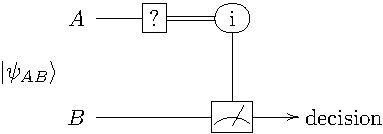
\includegraphics[width=0.9\linewidth]{gates1.pdf} 
	\caption{A schematic representation of the setup for distinguishing
		measurements by using entanglement. }
	\label{fig:scheme}
\end{figure}

\subsubsection{Theoretical results}



Let $M_{d_1,d_2}$ be the set of all matrices of dimension $d_1 \times d_2$ over
the field $\mathbb{C}$. For  simplicity notation, square matrices will be denoted by
$M_d$.  The subset of $M_d$ consisting of Hermitian matrices of dimension $d$ will  be  denoted  by $\HH_d$,  while  the  set  of  positive semidefinite matrices of dimension $d$ by $\HH_d^+$. The set of quantum states, that is positive semidefinite operators having
trace equal to one, will be denoted $\DD_d$.  The subset of $M_d$ consisting of unitary matrices will be denoted by
$\UU_d$, while its subgroup of diagonal unitary operators will be denoted by
$\DD \UU_d$.  An unitary transformation 
\todo[inline]{channel} CPTP 

$\Phi_{U}$ is defined as $\Phi_U(\cdot) := U \cdot U^\dagger$ for  $U \in \UU_d$. A general quantum
measurement, that is a positive operator valued measure (POVM) $\PP$ is a
collection of positive semidefinite operators $\{E_1, \ldots, E_m \}$ called
\emph{effects}, which sum up to identity, \ie $ \, \, \sum_{i=1}^m E_i = \1$. If
all the effects are rank-one projection operators, then such a measurement is
called von Neumann measurement. Every von Neumann measurement can be
parameterized by a unitary matrix and hence we will use the notation $\PP_{U}$
for a von Neumann measurement with effects $\{\proj{u_1}, \ldots, \proj{u_d}\}$,
where $\ket{u_i}$ is the $i$-th column of the unitary matrix $U$. The action of
quantum measurement $\PP_{U}$ on some state $\rho \in \mathcal{D}_d$ can be
expressed as the action of a quantum channel
$
\PP_{U} : \rho \rightarrow \sum_{i=1}^d \bra{u_i} \rho \ket{u_i} \proj{i}.
$ Every von Neumann measurement  $\PP_{U}$ can be also rewritten as $\Delta \circ \Phi_{(UE)^\dagger}$, where $\Delta$ denotes the completely dephasing channel.  








\subsubsection{Diamond norm}
Let us now consider linear mappings transforming  square matrices into square 
matrices 
that is \ $\Phi: M_{d_1} \to M_{d_2}$. 
 We define its completely bounded trace
norm, also known as a diamond norm, as
\begin{equation}
\|\Phi\|_\diamond = \max_{\|X\|_1=1} \| \left(\Phi \otimes \1\right) (X) \|_1.
\end{equation}


The celebrated result by Helstrom~\cite{helstrom1976quantum} gives an upper
bound on the probability of correct distinction between two quantum channels
$\Phi$ and $\Psi$ in terms of their distance with the use of the diamond norm
\begin{equation}
p \leq \frac12 + \frac14 \| \Phi - \Psi \|_\diamond.
\end{equation}


\begin{theorem}
Let $U\in \UU_d$ and let $\PP_U$ and $\PP_\Id$ be two von Neumann 
measurements. 
Let also 
$\diaguni_d$ be the set of diagonal unitary matrices of dimension $d$. Then
\begin{equation}
\|\PP_U - \PP_\Id\|_\diamond = \min_{E \in \diaguni_d} \|\Phi_{UE} - 
\Phi_\Id\|_\diamond,
\end{equation}
where $\Phi_U$ is unitary channel.
\end{theorem}


\paragraph{Discrimination of unitary channels}

Before we proceed to presenting our main results, we need to briefly discuss the
problem of discrimination of unitary channels. This can be done without the
usage of entangled input. In order to formulate the condition for perfect
discrimination of unitary channels we introduce the notion of numerical range of
a matrix $A \in M_d$, denoted by $W(A) =\{\bra{x}A\ket{x}: \ket{x} \in 
\mathbb{C}^d, \;
\;\braket{x}{x}=1\}$. The celebrated Hausdorf-T\"oplitz
theorem states that
$W(A)$ is a convex set and therefore $W(A) =\{\tr A \sigma : \sigma \in \Omega_d
\}$. Let us now recall the well-known result for the
distinguishability of unitary channels.
	Let $U \in \UU_d$ and $\Phi_U: \rho \mapsto U \rho U^\dagger$ be a unitary 
	channel. 
	Then 
	\begin{equation}
	\| \Phi_U  - \Phi_{\1} \|_\diamond = 2 \sqrt{1-\nu^2},
	\end{equation}
	where $\nu = \min_{x \in W(U^\dagger)} |x|  $. 

%\begin{proposition}
 Let $U = H_2 \diag(1, e^{i \phi}) H_2^\dagger$, $\phi \in [0, 2\pi)$ and	let 
 $\Phi_U$ and $\Phi_\Id$ be two unitary channels. The following equation holds 
	\begin{equation}
	\min_{E \in \diaguni_2} \|\Phi_{UE} - 
	\Phi_\Id\|_\diamond = \|\Phi_{U} - 
	\Phi_\Id\|_\diamond
	\end{equation}
%\end{proposition}


%In the general case, the diamond norm of a Hermiticity-preserving maps $\Phi$ 
%can be computed using the Semidefinite Program~\cite{watrous2018theory} and 
%state 
%primal and dual problem in the following form:	

%
%\begin{minipage}{0.495\linewidth}
%	\begin{equation*}
%		\begin{split}
%			\text{\textbf{Primal problem:}} \\
%			\text{maximize:}\quad & \tr(X J(\Phi)) \\[2mm]
%			\text{subject to:}\quad &  \left[ \begin{array}{cc}\Id_{d_2} \otimes \rho & X \\ X^* & \Id_{d_2} \otimes \rho  \end{array} \right] \ge 0 \\
%			& \rho \in \HH_d^+\\ 
%			& X \in M_{d1,d2}.
%		\end{split}
%	\end{equation*}
%\end{minipage}
%\begin{minipage}{0.495\linewidth}
%	\begin{equation*}
%		\begin{split}
%			\text{\textbf{Dual problem:}} \\
%			\text{minimize:}\quad & ||\tr_1(Y)||_\infty \\[2mm]
%			\text{subject to:}\quad & \left[ \begin{array}{cc}Y & -J(\Phi) \\ -J(\Phi) &  Y \end{array} \right] \ge 0 \\
%			& Y \in \HH_{d_1d_2}^+.
%		\end{split}
%	\end{equation*}
%	\vspace{0.5cm}
%\end{minipage} 


\subsubsection{Rigetti architecture's limits/ practical solutions}
\todo[inline]{nie wiem, moze tu o conditional measurement i o sposobach ominiecia tego problemu - postselekcja i kontrolowana unitarka}

We may encounter numerous obstacles in the implementation process due to the limited architecture of quantum computer. 
Let us take a closer look at the setup for distinguishing von Neumann 
measurements (see Fig.~\ref{fig:diamond}). One of the components of such a scheme is to perform the conditional binary measurement. The first limitation is lack to possibility of implementation of the conditional binary measurement. The only possible measurement performed on quantum architectures is measurement in the computational basis. 
A postselection method provides us with a clever going around the obstacle. The postselection  scheme (see Fig.~\ref{postselection})  can be described as follow. 


\begin{enumerate}
	\item We prepare input state $\ket{\psi_{AB}}$.
	\item One of two measurements is performed on part A.
	\item We prepare optimal measurements $V_j$, which are well known by Holevo--Helstrom theorem and perform them on part $B$.
	\item We get the output label $i$.
	\item We include these cases for which $i = j$. Otherwise, we reject them.
	\item By the use of $V_j$ output, we decide whether the measurement was performed on part $A$.
	\item We count the probability of postselection.
\end{enumerate}

\begin{figure}[h!]
	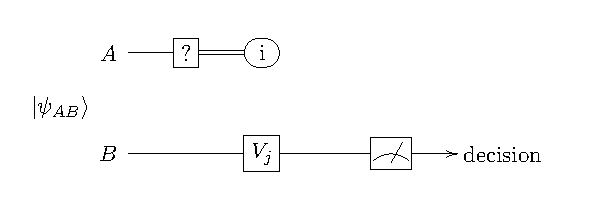
\includegraphics[scale=1.5]{onequbit.pdf}
	\caption{A schematic representation of the setup for distinguishing
		measurements using postselection.}
	\label{postselection}
\end{figure} 


\subsection{Sample code snippets analysis (optional)}
\todo[inline]{moze tu kod tej postselekcji  i kontrolowanej unitarki ? }
\label{}



\section{Illustrative Examples}

Let us focus on single-qubit von Neumann measurements $\PP_\1$ and $\PP_U$.
Assume that the unitary matrix $U$ is of the form 
\begin{equation}
U = H \diag (1, \ee^{\ii \phi}) H^\dagger,
\end{equation}
where $H$ is the Hadamard matrix of dimension two and $\phi \in [0, 2 \pi)$.
In this section we will compare theoretical probability of correct 
discrimination between these measurements and the realization on real devices.
The theoretical probability can be calculated using Holevo-Helstrom theorem. 
This probability will be calculated in 
subsection~\ref{sec:example_theoretical_probability}. Later, we will 
discuss the realization of this scheme on real devices in 
subsection~\ref{sec:example_realization}. For such realization, we 
will need the proper input state, (see sec.~\ref{sec:example_discriminator}) 
and final measurement (see sec.~\ref{sec_example_final_measurement}). 

\subsection{Theoretical bound}\label{sec:example_theoretical_probability}

\begin{proposition}
 Let $U = H \diag(1, e^{i \phi}) H^\dagger$, $\phi \in [0, 2\pi)$ and	let 
 $\Phi_U$ and $\Phi_\Id$ be two unitary channels. The following equation holds 
	\begin{equation}
	\min_{E \in \diaguni_2} \|\Phi_{UE} - 
	\Phi_\Id\|_\diamond = \|\Phi_{U} - 
	\Phi_\Id\|_\diamond
	\end{equation}
\end{proposition}
\begin{proof} We know that
$
	\| \Phi_U  - \Phi_{\1} \|_\diamond = 2 \sqrt{1-\nu^2},
$
	where $\nu = \min_{x \in W(U^\dagger)} |x|  $. For $U = H_2 \left(\begin{array}{cc}1&0\\0&e^{i \phi}\end{array}\right)  H_2^\dagger$ we obtain that $\nu = \frac{|1 + e^{i \phi} | }{2}$. 
	The condition $ 	\min_{E \in \diaguni_2} \|\Phi_{UE} - 
	\Phi_\Id\|_\diamond = \|\Phi_{U} - 
	\Phi_\Id\|_\diamond $ is equivalent to prove that
	\begin{equation}
	\max_{E \in \diaguni_2 } \nu_E = \nu = \frac{|1 + e^{i \phi} | }{2},
	\end{equation}
	where $\nu_E = \min_{x \in W(U^\dagger E)} |x|. $ We can prove that
	\begin{equation}
	\min_{\ket{x} \in \mathbb{C}^2  \proj{x} = 1} |\bra{x}U^\dagger\ket{x}| = \min_{\rho \in \Omega_2} |\tr(U^\dagger\rho)|. 
	\end{equation}
For that, to calculate $\nu_E$ we obtain \begin{equation}
	\max_{E \in \diaguni_2 } \nu_E  = \max_{E \in \diaguni_2 }  \min_{\rho \in \Omega_2} \left| \tr \rho U E  \right|
\end{equation}
For that, our task is reduce to show that
	\begin{equation}
	\forall E \in \diaguni_2 \,\, | \tr \rho U E | \le \nu. 
	\end{equation}
	Let us define $E = \left(\begin{array}{cc}E_0&0\\0&E_1\end{array}\right)  $ and let us take $\rho = \left(\begin{array}{cc}\frac{1}{2}&0\\0&\frac{1}{2}\end{array}\right) $. 
	From spectral theorem, let us note $U$ as
	\begin{equation}
	U= \lambda_1 \ketbra{x_1}{x_1} + \lambda_2 \ketbra{x_1}{x_2}, 
	\end{equation}
	where  for eigenvector $\lambda_1 = e^{\mathbf{i} \phi}$ the eigenvector is of the form $\ket{x_1} = \left[\begin{array}{c}\frac{1}{\sqrt{2}}\\-\frac{1}{\sqrt{2}}\end{array}\right]$, whereas for  $\lambda_2 = 1$ we have $\ket{x_2} = \left[\begin{array}{c}\frac{1}{\sqrt{2}}\\\frac{1}{\sqrt{2}}\end{array}\right]$.
	
	Then we have 
\begin{equation}
\begin{split}
& \forall E \in \diaguni_2 \,\,\, | \tr \rho U E | = \frac{1}{2}  \left| \tr H_2 \diag(1, e^{i\phi}) H_2^\dagger E \right| =  \\ &
\frac{1}{2} \left| \tr\left((  e^{i \phi} \proj{x_1} + 1 \proj{x_2} ) E \right) \right|  = 
\frac{1}{2} \left| e^{i \phi}  \bra{x_1} E \ket{x_1} + \bra{x_2} E \ket{x_2} \right| = \\& 
\frac{1}{2} \left| \frac{E_0 + E_1}{2} + e^{i \phi } \frac{E_0+E_1}{2} \right| = 
\frac{\left| 1+ e^{i \phi } \right|}{2} \left| \frac{E_0 + E_1}{2} \right| \le \nu, 
	\end{split}
\end{equation}
	which completes the proof.
\end{proof}


\begin{remark}
	The probability of correct discrimination of von Neumann measurements 
	$\PP_U$ and $\PP_{\Id}$ for $U = H_2 \diag(1, e^{i \phi}) H_2^\dagger$, 
	where $\phi \in [0, 2\pi)$ is given by
	\begin{equation}
	p \le \frac{1}{2} + \frac{|1 - e^{i \phi}  |}{4} . 
	\end{equation}
\end{remark}


\subsection{Realization}\label{sec:example_realization}

\subsubsection{Discriminator}\label{sec:example_discriminator}

\begin{theorem}\label{rozrpomiarow}
Let us $\mathcal{P}_U, \mathcal{P}_\1$ be two von Neumann measurements,  $U = H_2 \diag(1, e^{i \phi}) H_2^\dagger$, $\phi \in [0, 2\pi)$ such that $0 \not\in W(U)$.  If there exists the discriminator $\rho \in \Omega_2$ of the form $\rho = \frac{1}{2}\rho_1 + \frac{1}{2} \rho_2$ such that
	\begin{enumerate}
		\item $\rho_1,\rho_2 \in \Omega_2$
		\item $\Pi_1 \rho_1 \Pi_1 = \rho_1$,
		\item $\Pi_2 \rho_2 \Pi_2 = \rho_2$,
		\item  $\mathrm{diag}(\rho_1) = \mathrm{diag}(\rho_2)$,
	\end{enumerate}
	where $\Pi_1,\Pi_2 $ are the projectors on the subspaces
	spanned by the eigenvectors corresponding to $\lambda_1$ and $\lambda_2$ of $U$. Then  we have 
	\begin{equation}
	||\mathcal{P}_U - \mathcal{P}_\Id||_\diamond = 2\sqrt{1- \left|\frac{1+e^{i \phi}}{2}\right|^2}.
	\end{equation}
	%gdzie $\lambda_1, \lambda_n$ jest odpowiednio najmniejszą i największą wartością własną $U\in \mathrm{U}(\XX)$.
\end{theorem}
\begin{proof} From \ref{th:minE} we have 
	\begin{equation}
	\begin{split}
	||\mathcal{P}_U - \mathcal{P}_{\1}||_\diamond =\min_{E \in \diaguni_2} ||\mathcal{P}_{UE} - \mathcal{P}_{\1}||_\diamond = \min_{E \in \diaguni_2}|| \Delta \left(\Phi_{E^\dagger U^\dagger} - \Phi_{\1} \right) ||_\diamond \le \\ \le \min_{E \in \diaguni_2} ||\Delta||_\diamond || \Phi_{E^\dagger U^\dagger} - \Phi_{\1}  ||_\diamond \le \min_{\diaguni_2}|| \Phi_{E^\dagger U^\dagger} - \Phi_{\1} ||_\diamond.
	\end{split}
	\end{equation}
The diamond norm between two unitary channels can be calculated by 
	\begin{equation}
	\min_{E \in \diaguni_2}||\Phi_{E^\dagger U^\dagger} - \Phi_\1||_\diamond  = \min_{E \in \diaguni_2} 2\sqrt{1 - \min_{\rho \in \Omega_2} |\tr(UE \rho )|^2}.
	\end{equation}
Hence,  it is enough to calculate the formula
\begin{equation}
\begin{split}
\min_{E \in \diaguni_2} 2\sqrt{1 - \min_{\rho \in \Omega_2} |\tr(UE \rho )|^2}.
\end{split}
\end{equation}
Recall, let us note $U$ as
\begin{equation}
U= \lambda_1 \ketbra{x_1}{x_1} + \lambda_2 \ketbra{x_1}{x_2}, 
\end{equation}
where  for eigenvector $\lambda_1 = e^{\mathbf{i} \phi}$ the eigenvector is of the form $\ket{x_1} = \left[\begin{array}{c}\frac{1}{\sqrt{2}}\\-\frac{1}{\sqrt{2}}\end{array}\right]$, whereas for  $\lambda_2 = 1$ we have $\ket{x_2} = \left[\begin{array}{c}\frac{1}{\sqrt{2}}\\\frac{1}{\sqrt{2}}\end{array}\right]$. 
Consider two cases:

	$1^\circ$ Consider $\phi = \pi$. Then $U$ is of the form
	\begin{equation}
	U = \left(\begin{array}{cc}0&1\\1&0\end{array}\right).
	\end{equation}
Then $0 \in W(U)$. 	From Proposition 3 in ~\cite{puchala2018strategies} the measurements $\mathcal{P}_U, \mathcal{P}_\1$ are perfectly distinguishable if and only if there exists $\rho \in \Omega_2$ such that
	\begin{equation}
	\mathrm{diag}\left(U^\dagger \rho\right) = 0.
	\end{equation}
Hence, for $U $ we have 
	\begin{equation}
	0 = \mathrm{diag}\left(U^\dagger \rho\right) = \mathrm{diag} \left(\left(\begin{array}{cc}0&1\\1&0\end{array}\right)\left(\begin{array}{cc}\rho_{1,1}&\rho_{1,2}\\\rho_{2,1}&\rho_{2,2}\end{array}\right)\right) =  \mathrm{diag} \left(\begin{array}{cc}\rho_{2,1}&\rho_{2,2}\\\rho_{1,1}&\rho_{1,2}\end{array}\right).
	\end{equation}
 It implies that $\rho_{2,1}=\rho_{1,2} = 0$. Therefore $\rho \in \Omega_2$ for which $\mathcal{P}_U, \mathcal{P}_\1$  are perfectly distinguishable is of the form
	\begin{equation}
	\rho = \left(\begin{array}{cc}\rho_{1,1}&0\\0&\rho_{2,2}\end{array}\right),
	\end{equation}
	where $\rho_{1,1},\rho_{2,2} \ge 0$ and  $\rho_{1,1}+\rho_{2,2}=1$.

	$2^\circ$ Consider  $\phi \not = \pi$. 
The spectrum of $U$ is of the form $\sigma(U) = \{e^{\mathbf{i} \phi},1\}$. Hence $0 \not\in W\left(U\right)$.  Let us note $U$ as 
	\begin{equation}
	U= \lambda_1 \ketbra{x_1}{x_1} + \lambda_2 \ketbra{x_1}{x_2}.
	\end{equation}
Based on Lemma 5 in~\cite{puchala2018strategies} let us take $\rho_1 = \ketbra{x_1}{x_1}$ and $\rho_2 = \ketbra{x_2}{x_2}$. Obviously,  $\rho_1,\rho_2 \in \Omega_2$ and satisfies the requirements of theorem. Hence, the discriminator $\rho \in \Omega_2$ has the form 
	\begin{equation}
	\rho = \frac{1}{2} \rho_1 + \frac{1}{2}\rho_2 = \left(\begin{array}{cc}\frac{1}{2}&0\\0&\frac{1}{2}\end{array}\right)
	\end{equation}
%and 
%	\begin{equation}
%	||\mathcal{P}_U - \mathcal{P}_{\1}||_\diamond = 2 \sqrt{1 - \left| \frac{1 + e^{\mathbf{i} \phi}}{2}\right|^2 },
%	\end{equation}

	
%	
%	$1^\circ$ For $E = \1_\XX$ and $\rho  = \frac{1}{2} \rho_1 + \frac{1}{2} \rho_2$ we have 
%	\begin{equation}
%	\tr \left(U\rho \right) = \frac{1}{2} \lambda_1 \tr\left(\rho_1 \Pi_1 \right) + \frac{1}{2} \lambda_2 \tr\left(\rho_2\Pi_2 \right) = \frac{\lambda_1+\lambda_2}{2}. 
%	\end{equation}
%	Therefore, we have
%	\begin{equation}
%	2\sqrt{1 -  |\tr(UE \rho )|^2} =  2 \sqrt{1- \left|\frac{\lambda_1+\lambda_2}{2}\right|^2}.
%	\end{equation}
%	$2^\circ$ Let us consider  $E \in \diaguni_2$ given by $E = \sum_{i=1}^2 e_i \ketbra{i}{i}$   and $\rho  = \frac{1}{2} \rho_1 + \frac{1}{2} \rho_2$. Then we have 
%	\begin{equation}
%	\begin{split}
%	\tr \left(UE\rho \right) &= \frac{1}{2}\lambda_1 \tr \left(\rho_1 \Pi_1 E \right) + \frac{1}{2}\lambda_2 \tr \left(\rho_2 \Pi_2 E \right) = \\& = \frac{1}{2} \lambda_1 \sum_{i =1}^2 \bra{i}\rho_1 \ket{i} e_i + \frac{1}{2} \lambda_2 \sum_{i =1}^2 \bra{i}\rho_2 \ket{i} e_i = \frac{1}{2} \left(\lambda_1 + \lambda_2\right)\sum_{i=1}^2 \bra{i}\rho_1 \ket{i} e_i.
%	\end{split}
%	\end{equation} 
%So we have 
%	\begin{equation}
%	\left|\tr\left(UE \rho \right) \right| = \left|\frac{\lambda_1+\lambda_2}{2} \right| \cdot \left| \sum_{i=1}^2 \bra{i}\rho_2 \ket{i} e_i \right| \le \left|\frac{\lambda_1+\lambda_2}{2} \right|.
%	\end{equation}
%	It implies that
%	\begin{equation}
%	\sqrt{1 - \left|\frac{\lambda_1+\lambda_2}{2}\right|^2} \le \sqrt{1 -  |\tr(UE \rho)|^2} \le\sqrt{1 - \min_{\rho \in\Omega_2} |\tr(UE \rho )|^2}.
%	\end{equation}
%	Hence we obtain
%	\begin{equation}
%	\begin{split}
%	||\mathcal{P}_U - \mathcal{P}_{\1}||_\diamond &=  \max_{\rho \in \Omega_2} \sum_{i=1}^2  \sqrt{\left(\bra{u_i}\rho\ket{u_i} + \bra{i} \rho \ket{i} \right)^2 - 4|\bra{i}\rho\ket{u_i}|^2} \le \\& \le 2 \sqrt{1 -\left|\frac{\lambda_1+\lambda_2}{2} \right|^2}
%	\end{split}
%	\end{equation}
For $\rho =  \frac{1}{2} \rho_1 + \frac{1}{2} \rho_2$ we obtain
	\begin{equation}
	\begin{split}
	||\mathcal{P}_U - \mathcal{P}_{\1}||_\diamond &= \sum_{i=1}^2  \sqrt{\left(\bra{u_i}\rho\ket{u_i} + \bra{i} \rho \ket{i} \right)^2 - 4|\bra{i}\rho\ket{u_i}|^2} = \\& \sum_{i=1}^2  \sqrt{\left(\bra{i}U^\dagger\rho U \ket{i} + \bra{i} \rho \ket{i} \right)^2 - 4|\bra{i}\rho U \ket{i}|^2} = \\& \sum_{i=1}^2  \sqrt{4 \bra{i}\rho \ket{i}^2 - 4 \left| \frac{\lambda_1 \bra{i}\rho_1 \ket{i} + \lambda_2\bra{i} \rho_2\ket{i}}{2}\right|^2} =\\&  \sum_{i=1}^2  \sqrt{4 \bra{i}\rho \ket{i}^2 - 4 \bra{i} \rho \ket{i} \left| \frac{\lambda_1 + \lambda_2}{2}\right|^2} = \\&  \sum_{i=1}^2 2 \bra{i} \rho \ket{i} \sqrt{1 -\left| \frac{\lambda_1 + \lambda_2}{2}\right|^2 } = \\& 2 \sqrt{1 -\left| \frac{\lambda_1 + \lambda_2}{2}\right|^2 } = 
	2 \sqrt{1 -\left| \frac{1+e^{i \phi}}{2}\right|^2 } ,
	\end{split}
	\end{equation}
which completes the proof.
\end{proof}


\begin{remark}\label{lemma:rho}
	Let $\rho_{0} = \frac{1}{2} 
	\left(\begin{array}{cc}1&0\\0&1\end{array}\right)$. Then 
	\begin{equation}
	 \max_\rho \left\|(\1\otimes \sqrt{\rho}) J(\PP_U - \PP_{\Id}) 
	(\1\otimes 
	\sqrt{\rho})\right\|_1 =    \left\|(\1\otimes \sqrt{\rho_0}) J(\PP_U - 
	\PP_{\Id}) 
		(\1\otimes 
		\sqrt{\rho_0})\right\|_1
	\end{equation}
	for  $U = H_2\diag(1, e^{i \phi}) H_2^\dagger $, 
		where $\phi \in [0, 2\pi)$. 
\end{remark}


\subsubsection{Final measurement}\label{sec_example_final_measurement}
\begin{scheme}
Let us consider the problem of discrimination of von Neumann measurements 
$\PP_U$
and $\PP_{\Id}$ for $U = H_2 \diag(1, e^{i \phi}) H_2^\dagger$, 
	where $\phi \in [0, 2\pi)$. The schematic representation of theoretical 
	setup is shown in Fig.~\ref{fig:theoretical}. 

From ~\cite{puchala2018strategies}(Proposition 4) and Lemma~\ref{lemma:rho} we 
have 
	\begin{equation}
	\ket{\psi} = | \sqrt{\rho}^\top \rangle \rangle = \frac{1}{\sqrt{2}} |\Id_2 
	\rangle \rangle. 
	\end{equation}
	From Holevo-Helstrom theorem  we constrain a measurement $\mu$.  
	Let us define \begin{equation}
	X  = \left( \PP_U \otimes \Id_2 \right)(\proj{\psi}) -  \left( \PP_\Id 
	\otimes \Id_2 \right)(\proj{\psi})
	\end{equation}
	where $\ket{\psi}$ is defined in Remark~\ref{remark:discriminator}. From 
	Hahn-Jordan decomposition let \begin{equation}
	X = P - Q
	\end{equation}
	where $P, Q \ge 0 $. Observe, that $P $ and $Q$ are block-diagonal. 
	Let us define projectors $\Pi_P$ and $\Pi_Q$ onto  $im(P)$ and $im(Q)$, 
	respectively. Then  $\Pi_P$ and $\Pi_Q$ have the following forms
	\begin{equation}
	\Pi_P = \left(\begin{array}{cc}\proj{x_p}&0\\0&\proj{y_p}\end{array}\right) 
	\end{equation}
	and 
	\begin{equation}
	\Pi_Q = \left(\begin{array}{cc}\proj{x_q}&0\\0&\proj{y_q}\end{array}\right) 
	\end{equation}
	Hence, we define $V_0$ such that
	\begin{equation}
	\begin{split}
	V_0 \ket{x_p} = \ket{0} \\ 
	V_0 \ket{x_q} = \ket{1}
	\end{split}
	\end{equation}
	and $V_1$ such that
	\begin{equation}
	\begin{split}
	V_1 \ket{y_p} = \ket{0} \\ 
	V_1 \ket{y_q} = \ket{1}
	\end{split}
	\end{equation}
	The explicit form of $V_0$ and $V_1$ we can see in \texttt{one-qubit.nb}.
	Finally, we obtain the measurement $\mu$ of the form
	\begin{equation}
	\begin{split}
	 \mu(0) = \proj{0} \otimes V_0 \proj{0} V_0^\dagger +  \proj{1} \otimes V_1 
	 \proj{0} V_1^\dagger  \\ 
	\mu(1) = \proj{0} \otimes V_0 \proj{1} V_0^\dagger +  \proj{1} \otimes V_1 
	\proj{1} V_1^\dagger  
	\end{split}
	\end{equation}
\end{scheme}

%%%%%%%%%%%%%%%%%%%%%%%%%%%%%%%%%5



\paragraph{Construction of $V_0$ and $V_1$}
	For each $\phi \in \mathbb{R}$,  the controlled unitary $V_0$ and $V_1$ have the following form
	\begin{equation}
	V_0 = \left(\begin{array}{cc}i \sin\left( \frac{\pi - \phi}{4} \right)&-i \cos\left( \frac{\pi - \phi}{4} \right)\\ \cos\left( \frac{\pi - \phi}{4}\right)& \sin\left( \frac{\pi - \phi}{4} \right)\end{array}\right),
	\end{equation}
	
		\begin{equation}
	V_1 = \left(\begin{array}{cc}-i \cos\left(\frac{\pi - \phi}{4}\right) &i \sin\left( \frac{\pi - \phi}{4}\right)\\\sin\left( \frac{\pi - \phi}{4} \right) &  \cos\left( \frac{\pi - \phi}{4} \right) \end{array}\right).
	\end{equation}
	
\begin{scheme}(By using postsellection)

%\begin{figure}[h!]
%	\centering 
%	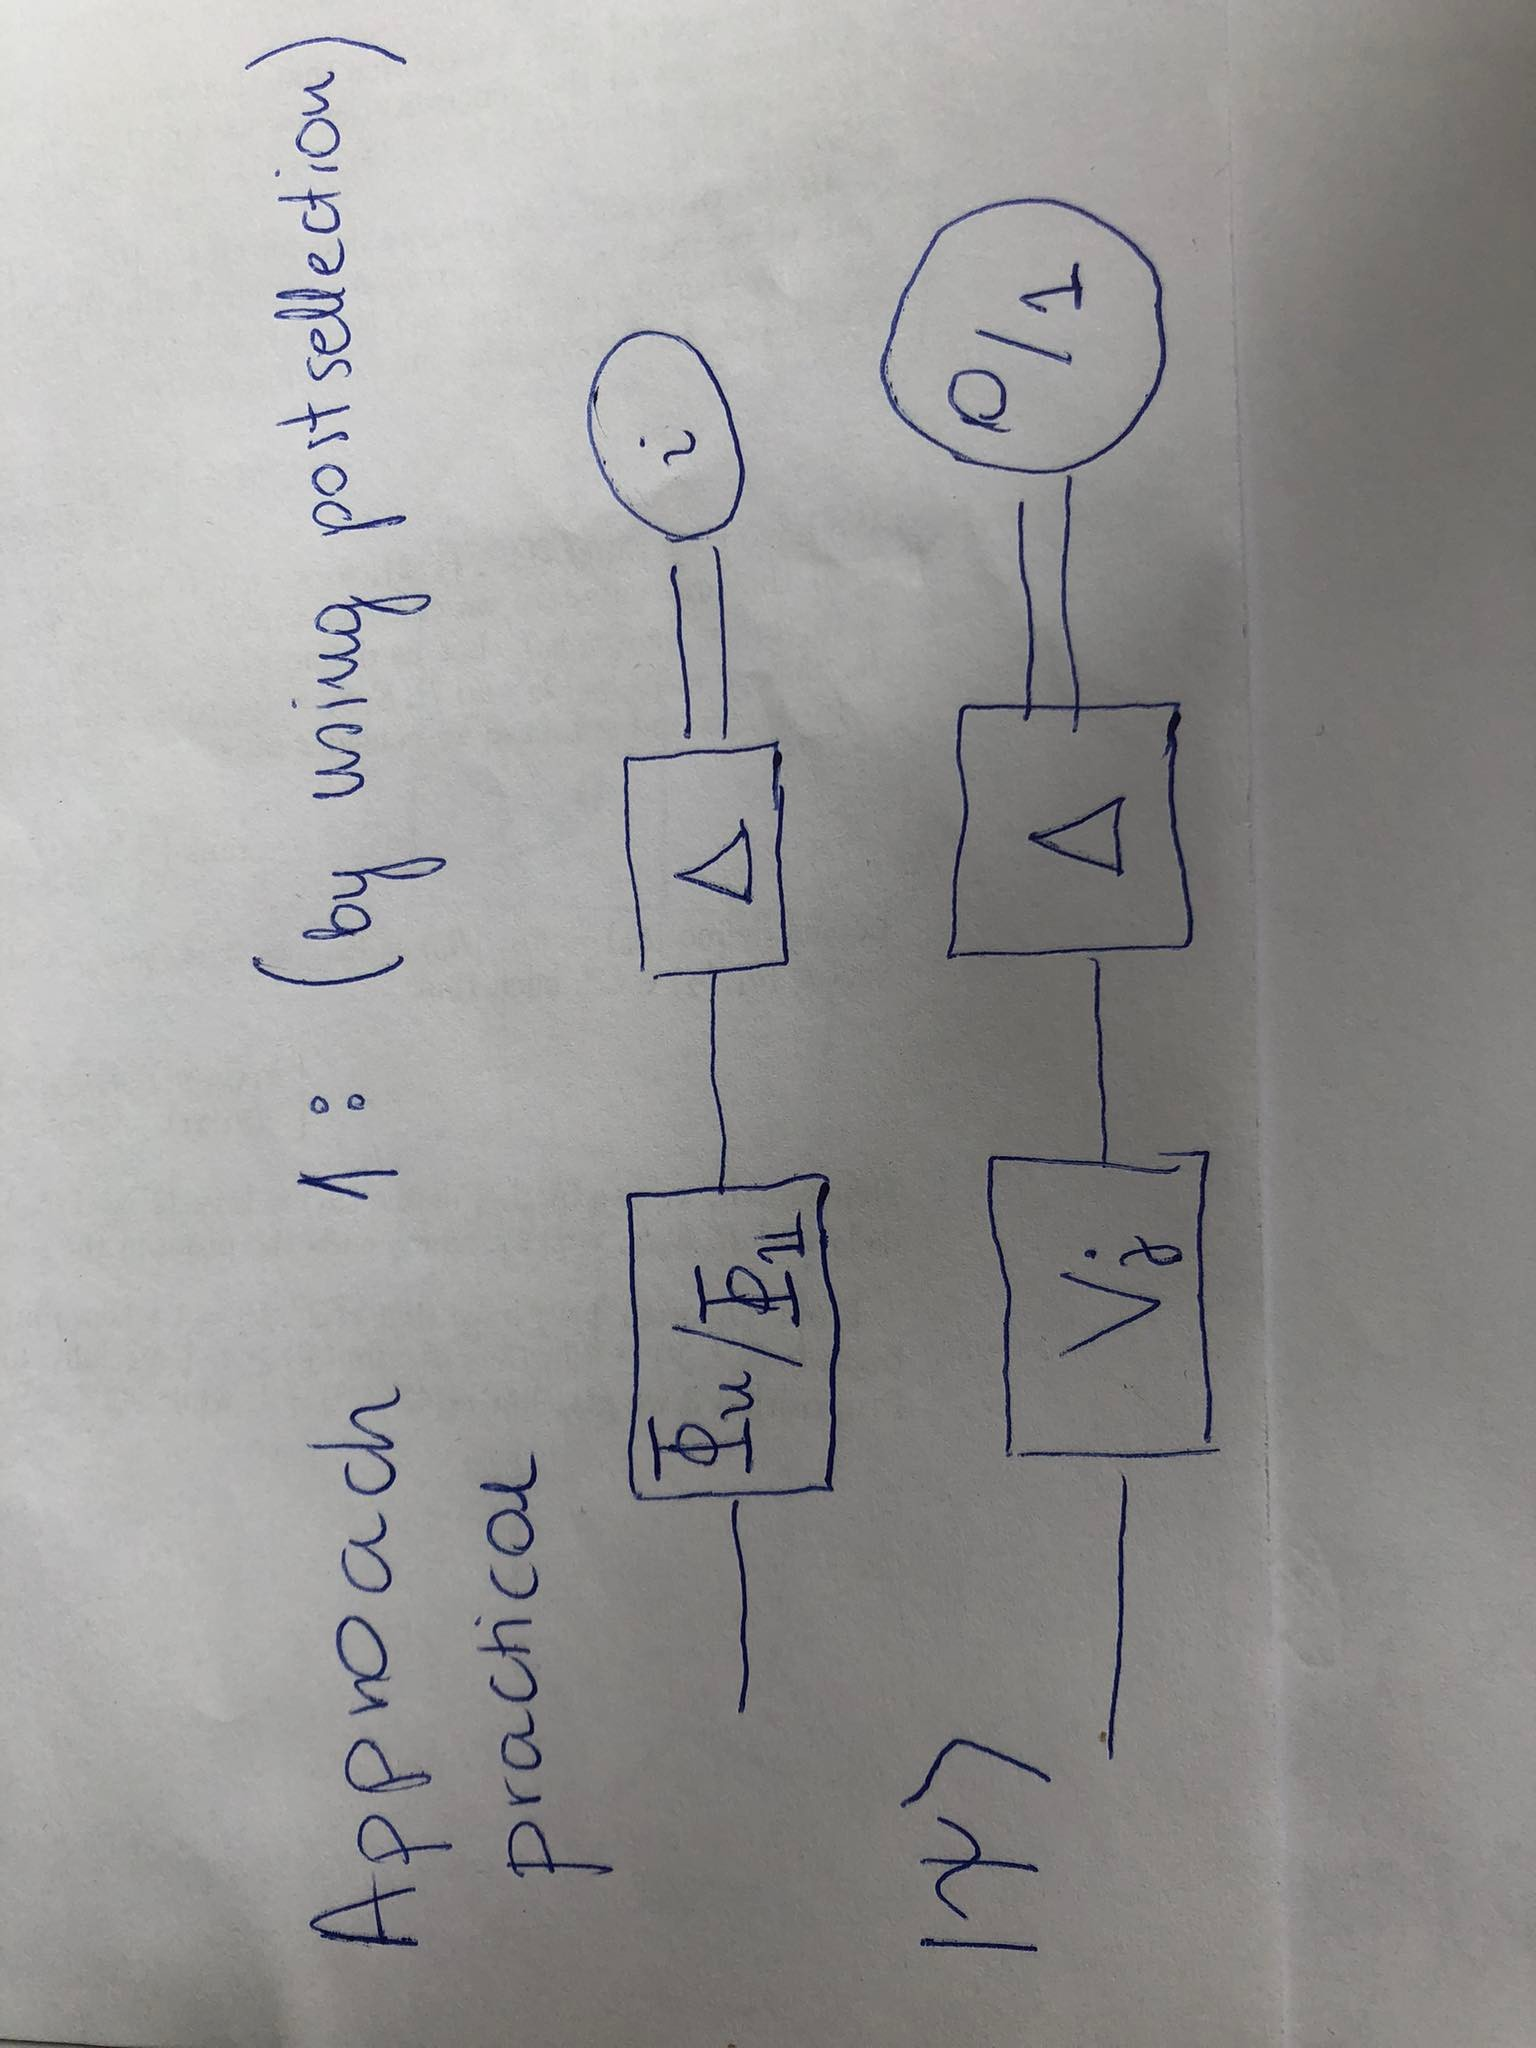
\includegraphics[width=0.75\linewidth, angle=-90]{rys-postsellection.jpg} 
%	
%	\caption{ A schematic representation of the setup for distinguishing
%		measurements using postselection. 
%	}\label{fig:postsellection}
%\end{figure}
\begin{enumerate}
\item We prepare input state $\ket{\psi} = \frac{1}{\sqrt{2} } | \Id_2 \rangle 
\rangle. $
\item We prepare one of two unitary channel $\Phi_{U} $ or $\Phi_{\1}$. 
\item We implement unitary $V_0 $ or $ V_1$.
\item We prepare the measurement $\Delta$ in standard basis (already exists on 
Rigetti architecture) on each qubits.
\item We calculate the probability of correct discrimination in the following 
way
\begin{equation}
p = ...
\end{equation}
%\todo[inline]{grubsza kmina, musze Ci to na zywo opowiedziec xd}
\end{enumerate}
\end{scheme}


\begin{scheme}(By using controlled unitary)
%\begin{figure}[h!]
%	\centering 
%	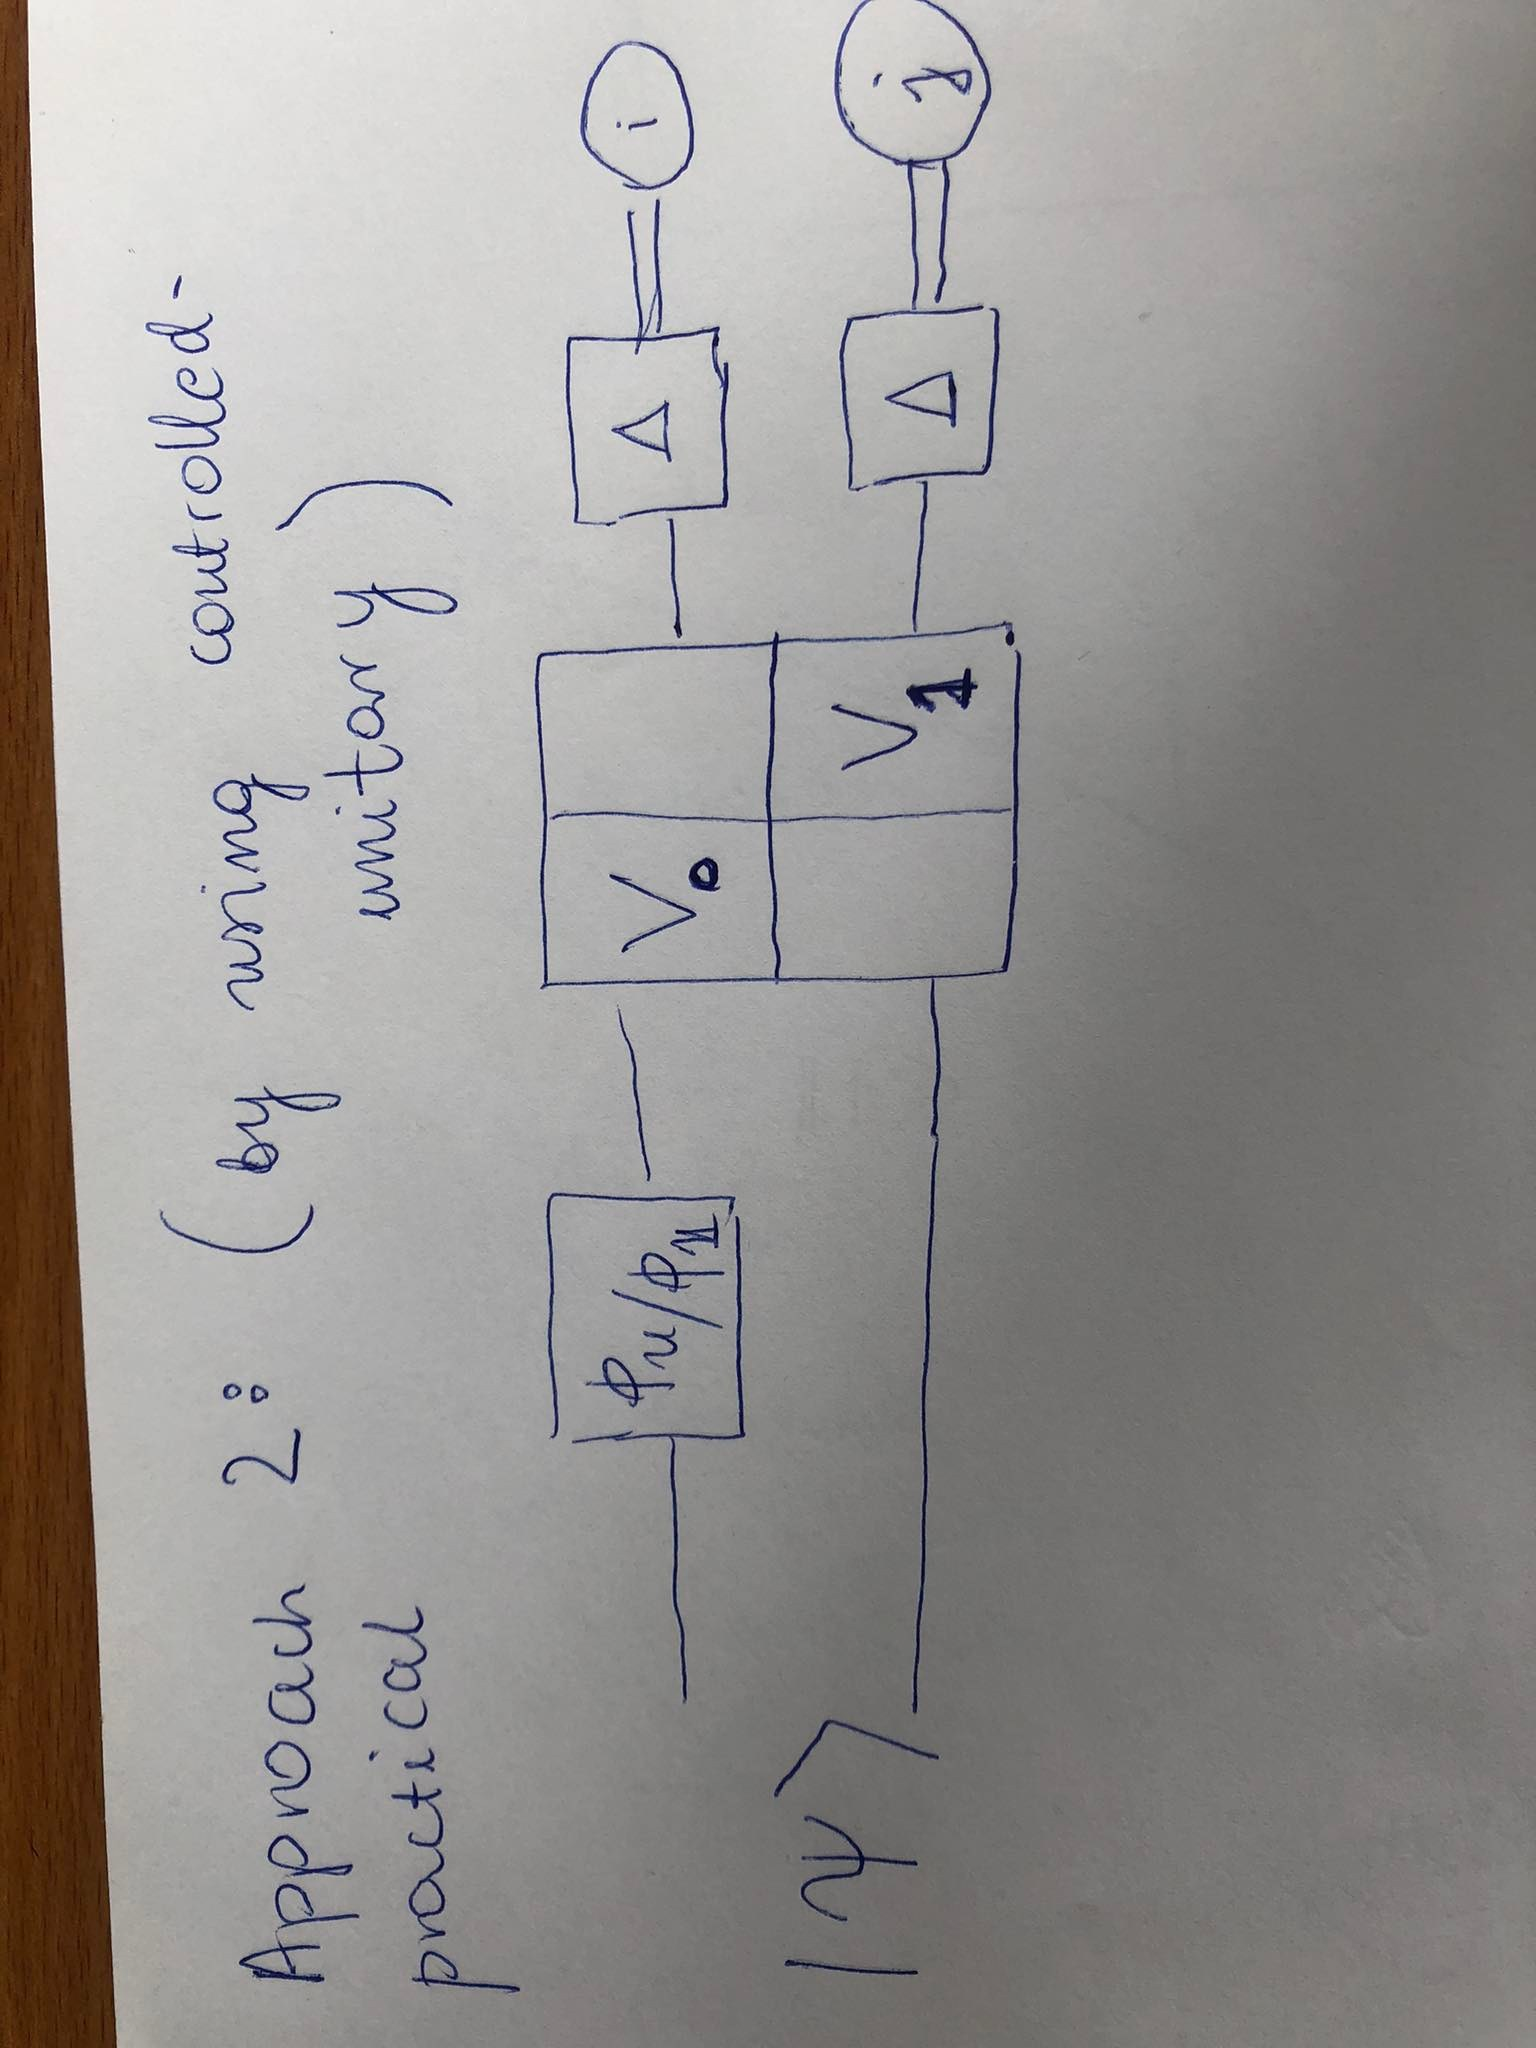
\includegraphics[width=0.75\linewidth, angle=-90]{rys-controlled.jpg} 
%	
%	\caption{ A schematic representation of the setup for distinguishing
%		measurements using controlled unitary gate. 
%	}\label{fig:controlled}
%\end{figure}
\begin{enumerate}
\item We prepare input state $\ket{\psi} = \frac{1}{\sqrt{2} } | \Id_2 \rangle 
\rangle. $
\item We prepare one of two unitary channel $\Phi_{U} $ or $\Phi_{\1}$. 
\item We implement controlled unitary $V_0 \oplus V_1$.
\item We prepare the measurement $\Delta$ in standard basis (already exist on 
Rigetti architecture) on each qubits.
\item We calculate the probability of correct discrimination in the following 
way
\begin{equation}
p = \frac{|j=0 \wedge \Phi_{U} | + |j=1 \wedge \Phi_{\1}|}{\text{all 
cases}}
\end{equation}
\end{enumerate}
\end{scheme}



%%%%%%%%%%%%%%%%%%%%%%%%%%%%%%%%%%

%Let us consider one-qubit von Neumann measurements $\PP_U$ and $\PP_\Id$. In 
%this simplest case,  we consider two von Neumann measurements $\PP_\1$ and 
%$\PP_U$ for $U = H_2 diag(0,\ee^{\ii \phi}) H_2$, where $H_d$--Hadamard matrix 
%of dimension $d$, $0 \le \phi < 2\pi$.    By theoretical results, the expected 
%probability $p_{success}$ of correct distinction between two measurements 
%$\PP_\1$ and $\PP_U$  is given by
%\begin{equation}
%p_{success} = \frac{1}{2} + \frac{1}{4} ||\PP_U - \PP_\1 ||_\diamond = 
%\frac{1}{2} + \frac{|1-\ee^{\ii \phi}|}{4}
%\end{equation}
%by the assumption the discriminator is on the form $\ket{\psi} = 
%\frac{1}{\sqrt{2}} ( \ket{00} +  \ket{11} )$. 
%(tu wyniki z rigettiego...)






\section{Impact }


\textbf{This is the main section of the article and the reviewers weight the description here appropriately}

Indicate in what way new research questions can be pursued as a result of the software (if any).

Indicate in what way, and to what extent, the pursuit of existing research questions is improved (if so).

Indicate in what way the software has changed the daily practice of its users (if so).

Indicate how widespread the use of the software is within and outside the intended user group.

Indicate in what way the software is used in commercial settings and/or how it led to the creation of spin-off companies (if so).

\section{Conclusions}
\label{}

Set out the conclusion of this original software publication.

\section{Conflict of Interest}
Please select the appropriate text:

Potential conflict of interest exists:
We wish to draw the attention of the Editor to the following facts, which may be considered as potential conflicts of interest, and to significant financial contributions to this work. The nature of potential conflict of interest is described below: [Describe conflict of interest]

No conflict of interest exists:
We wish to confirm that there are no known conflicts of interest associated with this publication and there has been no significant financial support for this work that could have influenced its outcome.


\section*{Acknowledgements}

This work was supported by the Foundation for Polish Science (FNP) under grant
number POIR.04.04.00-00-17C1/18-00.


% The Appendices part is started with the command \appendix;
% appendix sections are then done as normal sections
% \appendix

% \section{}
% \label{}

% References:
% If you have bibdatabase file and want bibtex to generate the
% bibitems, please use
%
%  \bibliographystyle{elsarticle-num} 
%  \bibliography{<your bibdatabase>}

% else use the following coding to input the bibitems directly in the
% TeX file.

\begin{thebibliography}{00}

\bibitem{preskill} Preskill, John. "Quantum Computing in the NISQ era and beyond." Quantum 2 (2018): 79.
\bibitem{michielsen2017benchmarking} Michielsen, Kristel, et al. "Benchmarking gate-based quantum computers." Computer Physics Communications 220 (2017): 44-55.
\bibitem{zhukov2019quantum} Zhukov, A. A., et al. "Quantum communication protocols as a benchmark for programmable quantum computers." Quantum Information Processing 18.1 (2019): 1-23.
\bibitem{hamilton2018generative} Hamilton, Kathleen E., Eugene F. Dumitrescu, and Raphael C. Pooser. "Generative model benchmarks for superconducting qubits." Physical Review A 99.6 (2019): 062323.
\bibitem{benedetti2018generative} Benedetti, Marcello, et al. "A generative modeling approach for benchmarking and training shallow quantum circuits." npj Quantum Information 5.1 (2019): 1-9.
\bibitem{puchala2018strategies} Puchała, Zbigniew, et al. "Strategies for optimal single-shot discrimination of quantum measurements." Physical Review A 98.4 (2018): 042103.
\end{thebibliography}
\todo[inline]{Please add the reference to the software repository if DOI for software  is available. }

\section*{Current executable software version}
\label{}

Ancillary data table required for sub version of the executable software: (x.1, x.2 etc.) kindly replace examples in right column with the correct information about your executables, and leave the left column as it is.

\begin{table}[!h]
\begin{tabular}{|l|p{6.5cm}|p{6.5cm}|}
\hline
\textbf{Nr.} & \textbf{(Executable) software metadata description} & \textbf{Please fill in this column} \\
\hline
S1 & Current software version & For example 1.1, 2.4 etc. \\
\hline
S2 & Permanent link to executables of this version  & For example: $https://github.com/combogenomics/$ $DuctApe/releases/tag/DuctApe-0.16.4$ \\
\hline
S3 & Legal Software License & List one of the approved licenses \\
\hline
S4 & Computing platforms/Operating Systems & For example Android, BSD, iOS, Linux, OS X, Microsoft Windows, Unix-like , IBM z/OS, distributed/web based etc. \\
\hline
S5 & Installation requirements \& dependencies & \\
\hline
S6 & If available, link to user manual - if formally published include a reference to the publication in the reference list & For example: $http://mozart.github.io/documentation/$ \\
\hline
S7 & Support email for questions & \\
\hline
\end{tabular}
\caption{Software metadata (optional)}
\label{} 
\end{table}

\end{document}
\endinput
%%
%% End of file `SoftwareX_article_template.tex'.
